\part{Turing machines}
\frame{\partpage}

\begin{frame}{Turing machines}
    \begin{center}
        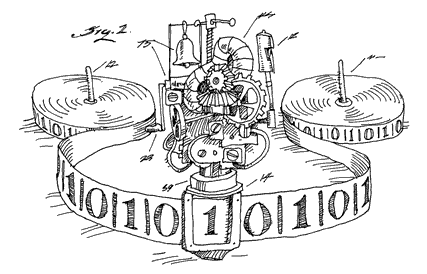
\includegraphics[width=0.6\textwidth]{turing_machine}
        % Image from https://medium.com/@calhoun137/alan-turings-universal-computing-machine-be69c052c6fd
    \end{center}
    \begin{itemize}
        \pause\item Introduced in 1936 by Alan Turing
        \pause\item Theoretical model of a ``computer''
            \begin{itemize}
                \pause\item I.e.\ a machine that carries out computations (calculations)
            \end{itemize}
    \end{itemize}
\end{frame}

\begin{frame}{Turing machine}
    \begin{itemize}
        \pause\item Has a finite number of \textbf{states}
        \pause\item Has an infinite \textbf{tape}
        \pause\item Each space on the tape holds a \textbf{symbol} from a finite \textbf{alphabet}
        \pause\item Has a \textbf{tape head} pointing at one space on the tape
        \pause\item Has a transition table which, given:
            \begin{itemize}
                \pause\item The current state
                \pause\item The symbol under the tape head
            \end{itemize}
        \pause specifies:
            \begin{itemize}
                \pause\item A new state
                \pause\item A new symbol to write to the tape, overwriting the current symbol
                \pause\item Where to move the tape head: one space to the left, or one space to the right
            \end{itemize}
    \end{itemize}
\end{frame}

\begin{frame}{The Church-Turing Thesis}
    \begin{itemize}
        \pause\item If a calculation can be carried out by a mechanical process at all,
            then it can be carried out by a Turing machine
        \pause\item I.e.\ a Turing machine is the most ``powerful'' computer possible,
            in terms of what is possible or impossible to compute
        \pause\item A machine, language or system is \textbf{Turing complete} if it can simulate a Turing machine
        \pause\item (In practice, nothing can simulate an infinite tape, so we just assume a large enough tape)
    \end{itemize}
\end{frame}

\begin{frame}{Examples of Turing complete systems}
    \begin{itemize}
        \pause\item All general-purpose CPUs and programming languages
        \pause\item Esoteric programming languages (e.g. Brainf*ck)
        \pause\item NAND gate circuits
        \pause\item Cellular automata
        \pause\item Minecraft redstone circuits
        \pause\item Factorio circuit networks
        \pause\item Magic: The Gathering cards
        \pause\item ...
    \end{itemize}
\end{frame}

